\chapter{Introduction}	% The first Chapter.
Quantum-confined semiconductor nanocrystals (NCs) are crystalline clusters of atoms having a semiconductor composition with diameters smaller than the spatial extent of the electron and/or hole wavefunction in the corresponding bulk material. In this case, that particular carrier is said to be experiencing quantum confinement. While such materials are also commonly referred to as quantum dots, we refer to this material class (colloidal, quantum confined semiconductor nanocrystals) as NCs to distinguish them from the various other types of quantum dots common in the literature, such as epitaxial self-assembled quantum dots or gate-defined quantum dots. In this thesis, we focus on cluster sizes and materials for which \emph{both} carriers are strongly confined. In general, NCs exhibit size-dependent, broadly tunable absorption and emission spectra, near-unity quantum yields, and are amenable to low-cost, easily scalable solution-phase processing. Furthermore, they exhibit emergent physical processes such as hot electron transfer and carrier multiplication. As a result, they have been suggested as a means to improve a wide variety of energy-relevant technologies including LEDs, lasers, solar cells, transistors, and thermoelectric power converters. Since their initial synthesis in 1985, the optical and electronic properties of NCs have received a great deal of attention, and a great deal is now understood regarding the electronic structure of this fascinating material class. We review some important aspects of NC electronic structure and optical properties here. As the work presented in this thesis is concerned with nanoscale energy generation and dissipation, we also review the basics of phonon-assisted carrier cooling and thermal transport.

\section{Quantum Confinement and Electronic Structure}
\subsection{Particle-in-a-Sphere}
The remarkable effects of quantum confinement are most easily understood by considering the NC as a particle-in-a-sphere \cite{efros1982interband, brus1986electronic}, analogous to the particle-in-a-box problem familiar from quantum mechanics. We will begin by applying spherical boundary conditions to a bulk semiconductor wavefunction. The spherical boundary conditions applied here take the form of an infinite spherical potential of radius $a$, $V(\vec{r})$, such that:
\begin{equation}\label{eq:pis1}
V(\vec{r}) = \left\{
	\begin{array}{ll}
		0 & \mbox{if } \vec{r} < a \\
		\infty & \mbox{if } \vec{r} > a
	\end{array}
\right.
\end{equation}

As a starting point, we utilize Bloch's theorem, which states that in a perfectly crystalline and periodic material, we may write the carrier wavefunction as the product of a wavelike portion and a cell-periodic portion, as shown below:
\begin{equation}\label{eq:pis2}
\Psi_{n\vec{k}}(\vec{r}) = u_{n\vec{k}}e^{i\vec{k}\cdot\vec{r}}
\end{equation}
In Equation \ref{eq:pis2}, the function $u_{n\vec{k}}$ is a function with the periodicity of the crystal lattice, with the wavefunctions being labeled by band index $n$ and wavevector $\vec{k}$. Eigenvalues of the Schr{\"o}dinger equation for Eq. \ref{eq:pis2} yield an energy spectrum of the form:
\begin{equation}\label{eq:pis3}
E_{n}\left(\vec{k}\right) = \frac{\hbar^2\vec{k}_n^2}{2m_{\mathrm{eff}}}
\end{equation}
In Eq. \ref{eq:pis3} we have utilized the so-called effective mass approximation, in which semiconductor carriers behave as free particles but with an altered ("effective") mass compensating for the complex potential experienced by the carriers due to the host lattice. In the effective mass approximation, the valence and conduction bands are assumed to have parabolic forms, evident in the $\vec{k}^2$ dependence of the energy levels (Eq. \ref{eq:pis3}) and demonstrated graphically in Figure \ref{f:pis1}. \par

\begin{figure}
\begin{center}
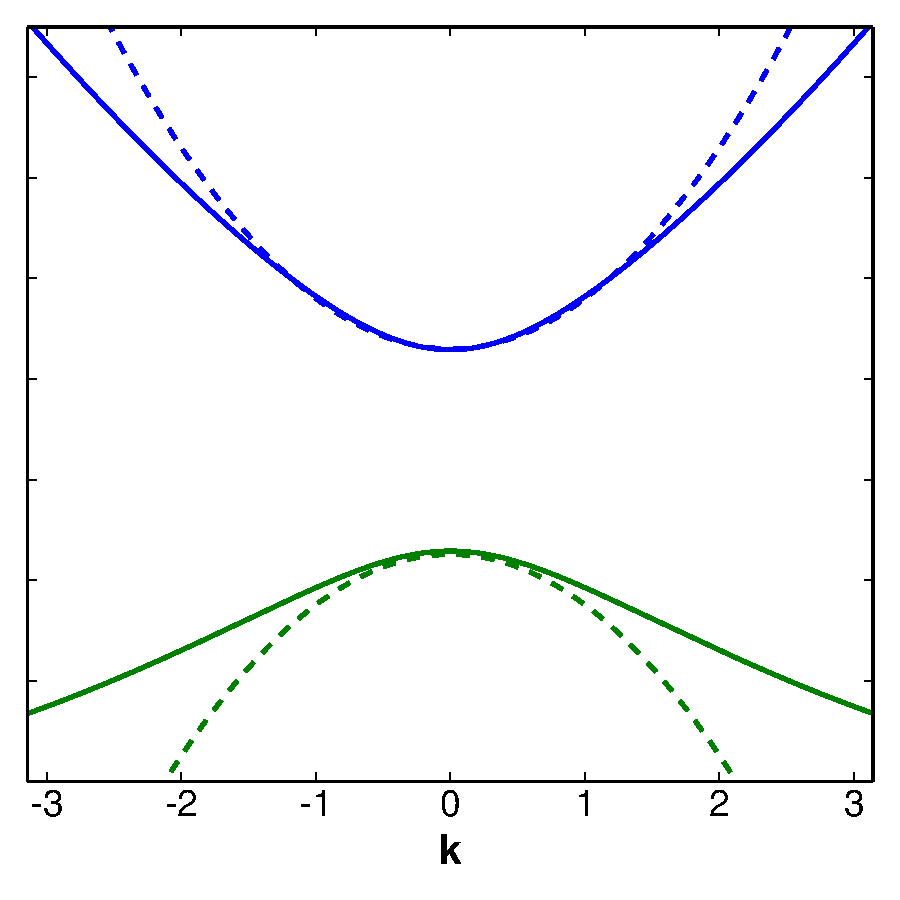
\includegraphics[width=0.5\textwidth]{./Chapter1/parabolic.pdf}
\caption[Two-band model for a direct gap semiconductor in the parabolic band approximation.]{Two-band model for a direct gap semiconductor in the parabolic band approximation. The true band structure is shown in solid lines, while the parabolic bands, centered at $\vec{k} = 0$ utilized in the effective mass approximation are shown in dashed lines.}
\label{f:pis1}
\end{center}
\end{figure}

To satisfy the spherical boundary condition, the single-particle (i.e. electron or hole) wavefunction is written as a linear combination of Bloch wavefunctions (Eq. \ref{eq:pis2}):
\begin{equation}\label{eq:pis4}
\Psi_{sp}\left(\vec{r}\right) = u_{n0}\left(\vec{r}\right)\sum_{\vec{k}}C_{n\vec{k}}e^{i\vec{k}\cdot\vec{r}}
\end{equation}
In Eq. \ref{eq:pis4}, we have assumed no dependence of $u$ on $\vec{k}$, implying a tight-binding approximation and allowing the function $u$ to be written as a sum of atomic wavefunctions $\{\phi\}$, i.e. $u_n \approx \sum_{i} C_{ni}\phi_n\left(\vec{r} - \vec{r_i}\right)$ where $i$ indexes the lattice sites. This reduces the problem to the determination of the envelope functions, $f_{sp}\left(\vec{r}\right) = \sum_{\vec{k}}C_{n\vec{k}}e^{i\vec{k}\cdot\vec{r}}$, which enforce the spherical symmetry. These envelope functions can be calculated by solving the Schr{\"o}dinger equation for an arbitrary particle in a spherical confining potential (Eq. \ref{eq:pis1}). This yields wavefunctions of the form:
\begin{equation}\label{eq:pis5}
\Phi_{n,l,m}\left(r,\theta, \phi\right) = C\frac{j_l\left(k_{n,l},\vec{r}\right)Y_l^m\left(\theta,\phi\right)}{r}
\end{equation}
In Eq. \ref{eq:pis5}, $Y_l^m\left(\theta,\phi\right)$ is a spherical harmonic function, $j_l\left(k_{n,l},\vec{r}\right)$ is the $l$th order spherical Bessel function, and $k_{n,l} = \alpha_{n,l}/a$, where $\alpha_{n,l}$ is the $n$th zero of $j_l$. Plugging the functions $\Phi$ directly in for the envelope functions $f_{sp}$, we arrive at the electron-hole pair states:
\begin{equation}\label{eq:pis6}
\begin{split}
\Psi_{e-h}\left(\vec{r}_e, \vec{r}_h\right) &= \Psi_e\left(\vec{r}_e\right)\Psi_h\left(\vec{r}_h\right) = u_ef_e\left(\vec{r}_e\right)u_hf_h\left(\vec{r}_h\right) \\
&= C\left[u_e\frac{j_{Le}\left(k_{ne,Le},\vec{r}_e\right)Y_l^m\left(\theta,\phi\right)}{r}\right]\left[u_h\frac{j_{Lh}\left(k_{nh,Lh},\vec{r}_h\right)Y_l^m\left(\theta,\phi\right)}{r}\right]
\end{split}
\end{equation}
Solving for the eigenvalues associated with these wavefunctions and adding offsets to account for the bulk semiconductor band gap ($E_g$) and Coulomb interaction of the electron and hole ($E_c$) yields the energy eigenvalues for the electron-hole pairs:
\begin{equation}\label{eq:pis7}
E_{e-h} \left(n_h, L_h, n_e, L_e\right) = E_g + \frac{\hbar^2}{2a^2}\left(\frac{\alpha_{nh, Lh}^2}{m_{\mathrm{eff}}^h} + \frac{\alpha_{ne, Le}^2}{m_{\mathrm{eff}}^e}\right) - E_c
\end{equation}
In Eqs. \ref{eq:pis6} and \ref{eq:pis7}, the quantum states are labeled by the quantum numbers $n_h, L_h, n_e$, and $L_e$. While the bookkeeping begins to become cumbersome, Eqs. \ref{eq:pis6} and \ref{eq:pis7} reveal some important basic features of NC electronic structure. Firstly, the enforcement of spherical boundary conditions leads to a quantization of the wavevector $k$, yielding a discrete, molecule-like density of states. Figure \ref{f:pis2} graphically depicts the quantization of $k$ values and resulting set of discrete transitions. Furthermore, the dependence of $E_{e-h}$ on $a^{-2}$ reveals the strongly size-dependent energy spectra characteristic to NCs. Finally, it is worth noting that the simple treatment of electron-hole Coulomb attraction as a first-order correction to the energy is justified in this case: Confinement energy ($\propto a^{-2}$) overwhelms the Coulomb interaction ($\propto a^{-1}$) in the strong confinement regime. It is worth noting that while the term "exciton" is occasionally used in this thesis to refer to NC electron-hole pairs, this terminology is used loosely with the full understanding that these excitons are most strongly bound by spatial confinement rather than Coulombic attraction, in contrast to the excitons found in bulk materials. Still, theoretical treatments of the strongly-confined electron-hole pair as a single exciton quasiparticle have been found to be effective for describing many properties of interest \cite{scholes2006excitons}. \par

\begin{figure}
\begin{center}
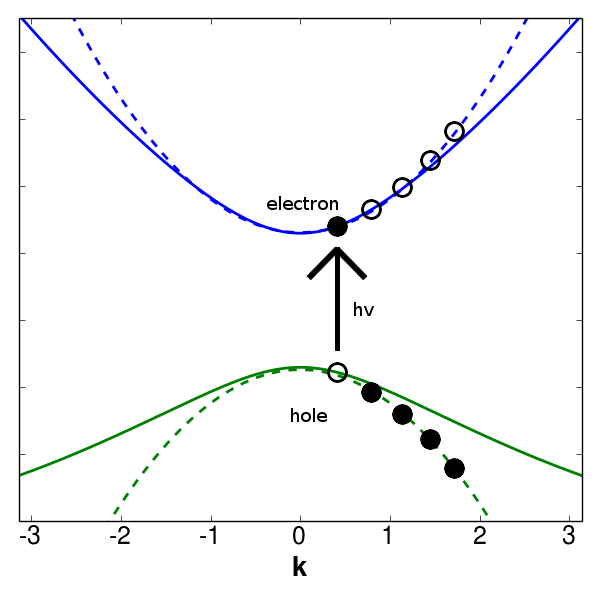
\includegraphics[width=0.5\textwidth]{./Chapter1/parabolic_quantized.png}
\caption[Discrete energy spectrum in a two-band model due to spherical confinement.]{Discrete energy spectrum in a two-band model due to spherical confinement. Imposing a spherical confining potential on the bulk Bloch wavefunctions results in $k$ quantization, with each electron/hole shown in the figure representing a quantized $k$ state.}
\label{f:pis2}
\end{center}
\end{figure}

\subsection{Exciton Fine Structure}
While the particle-in-a-sphere model is useful for understanding the physical origins of discrete transitions and size-dependent optoelectronic properties in NCs, the band structure of real semiconductor compositions is significantly more complicated. As an example, CdSe, an archetypal semiconductor nanocrystal composition, is a $sp^3$ hybridized semiconductor exhibiting the wurtzite crystal structure. Se $4p$ orbitals form the valence band, while Cd $5s$ orbitals form the conduction band. As both Cd and Se are relatively heavy elements, CdSe NCs exhibit strong spin orbit coupling, which splits the valence band into a fourfold degenerate band maximum and a split-off sub-band. Another consequence of this strong spin-orbit coupling is that only the total angular momentum of a state $F$ (spin + orbital momentum) is a good quantum number. Because excited electrons occupy $s$ orbitals, they exhibit $F_{\mathrm{electron}} = \pm1/2$, while valence band ($p$-orbital) holes may exhibit $F_{\mathrm{hole}} = \pm3/2$ or $\pm1/2$. Therefore an electron-hole pair may have $F = \pm2, \pm1$ or 0. The lowest excitonic state of CdSe NCs presents eight fine structure states, two having $F = \pm2$, four having $F= \pm1$, and two having $F = 0$. Figure \ref{f:efs1} displays a schematic of this excitonic state in terms of the exciton fine structure described here. \par

\begin{figure}
\begin{center}
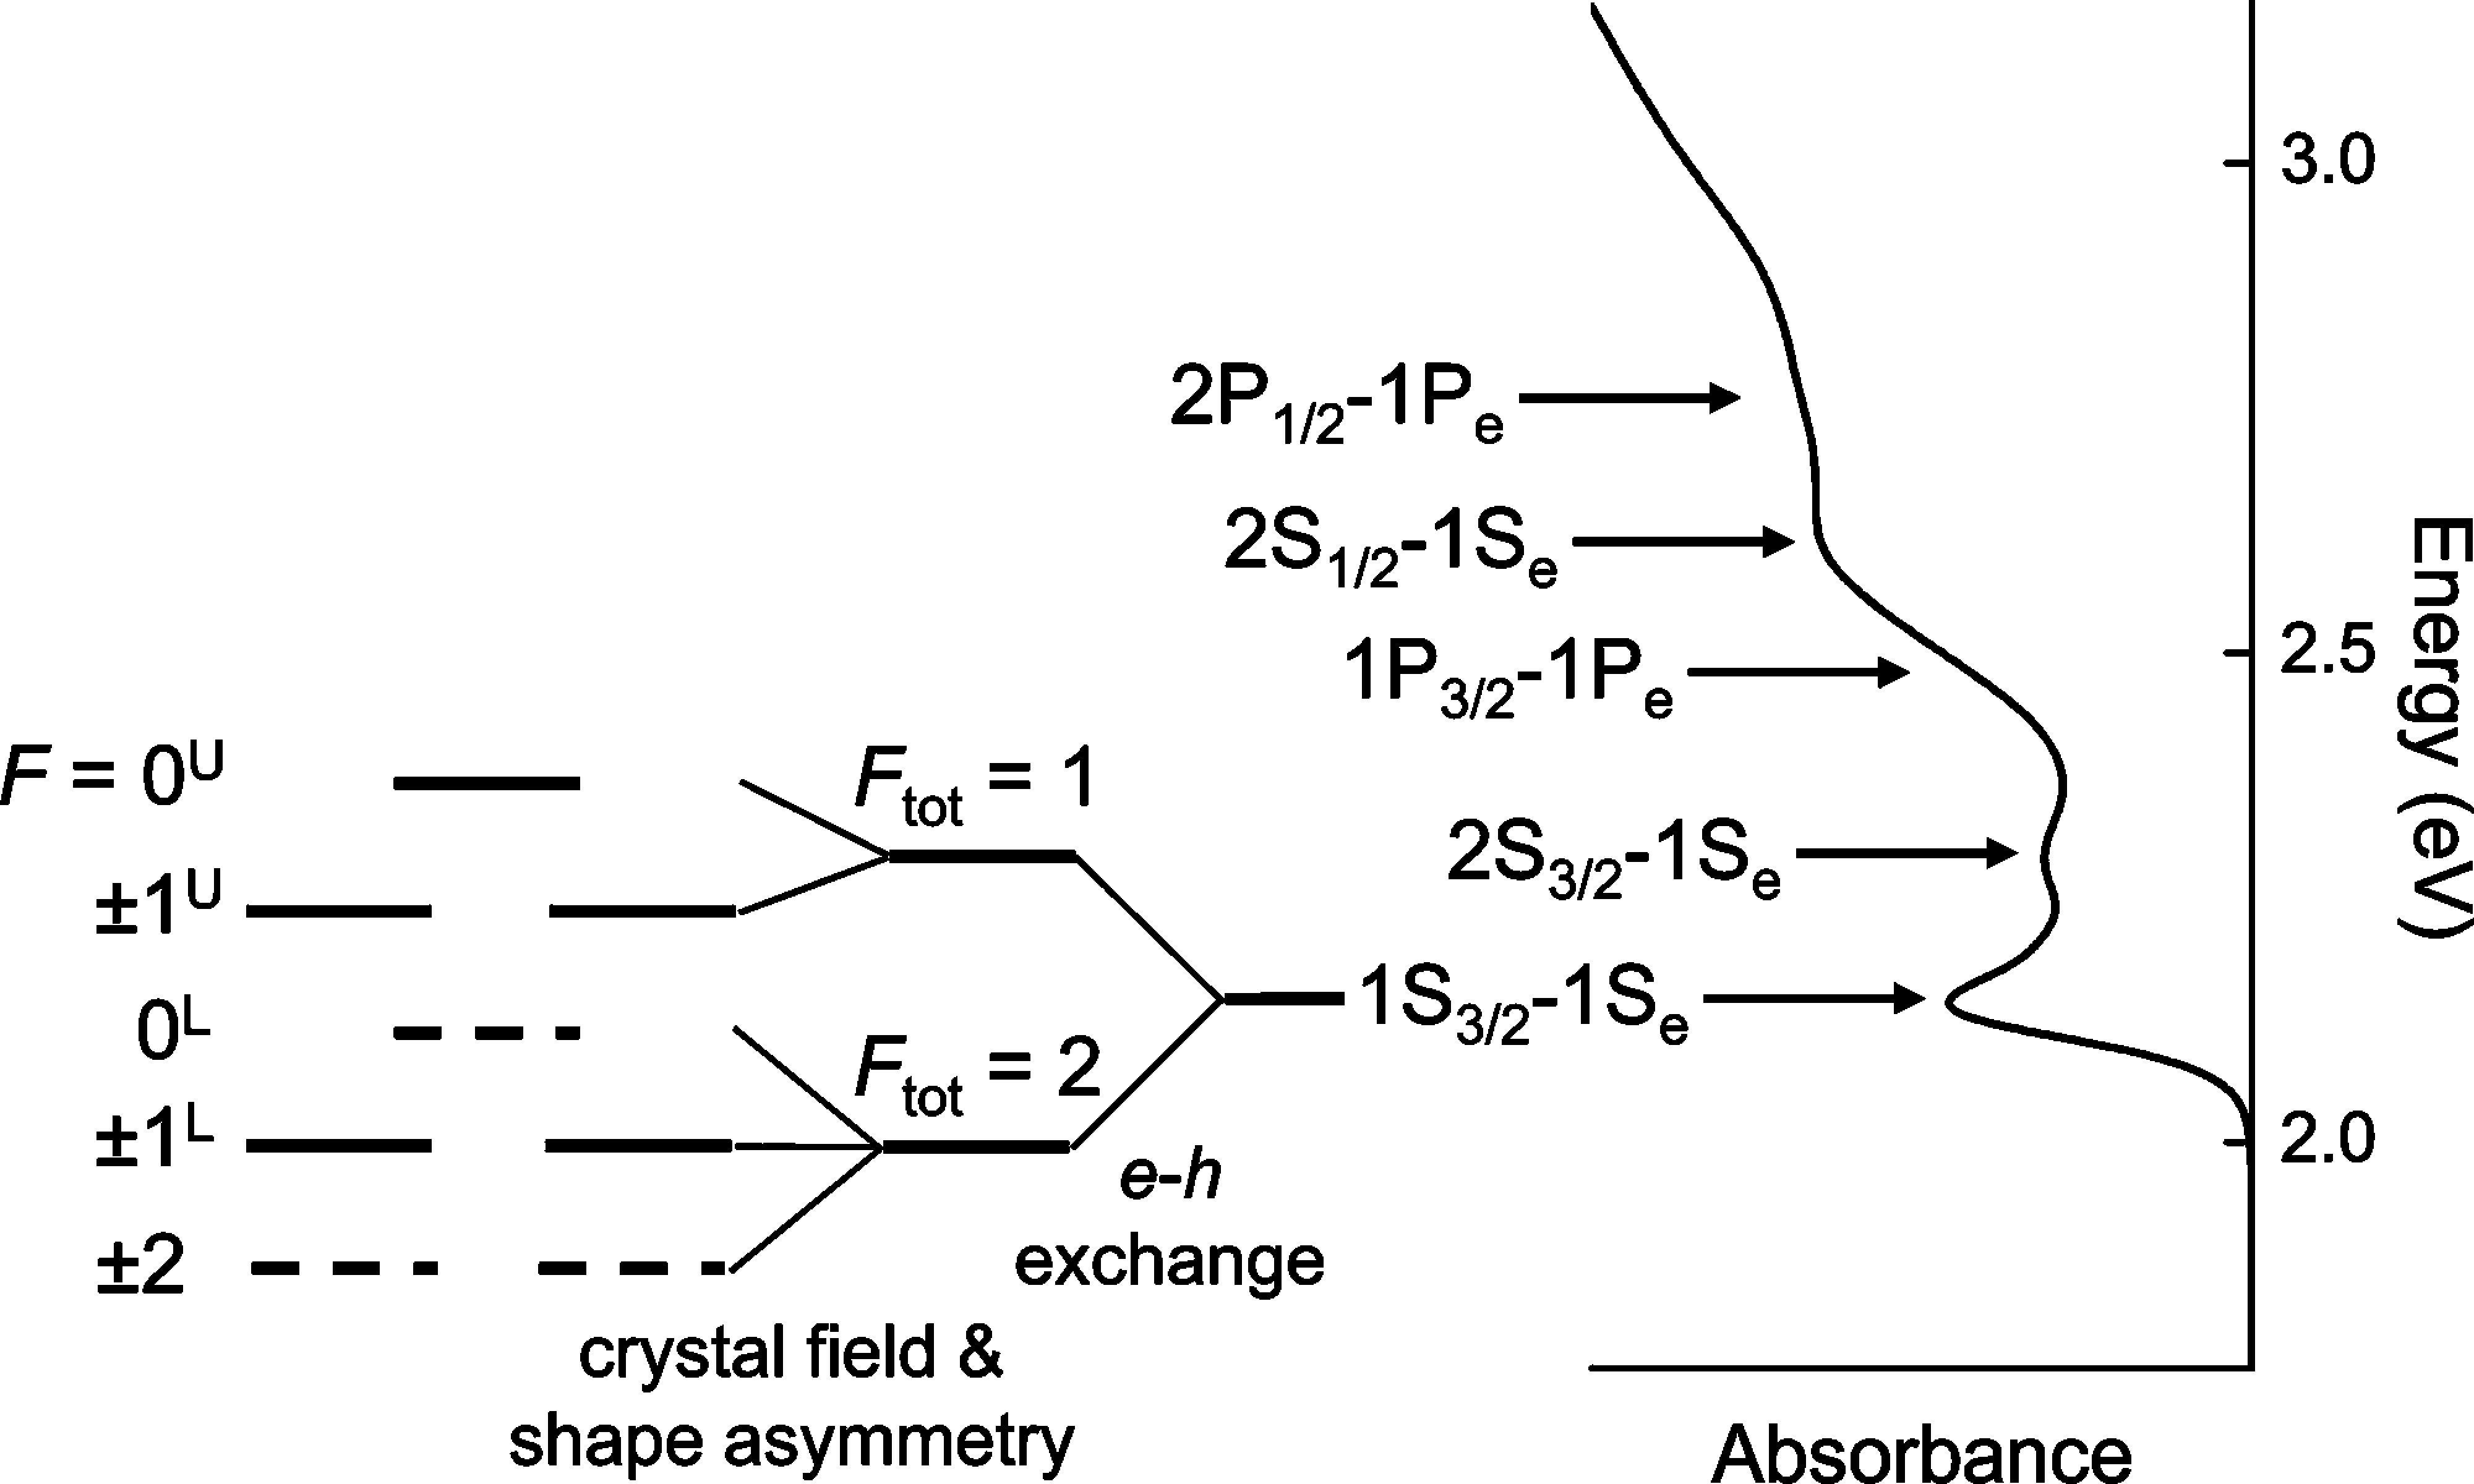
\includegraphics[width=\textwidth]{./Chapter1/efs_scholes.jpeg}
\caption[Exciton fine structure of CdSe nanocrystals]{Optical absorption spectrum of CdSe NCs (right hand side) with the first sharp absorption peak, due to the lowest-energy excitonic state $1S_{3/2}-1S_e$, labeled according to its exciton fine structure states \cite{kim2009exciton}.}
\label{f:efs1}
\end{center}
\end{figure}

Another consequence of spatial confinement is that the exchange interaction between electrons and holes become greatly enhanced. In brief, the exchange interaction causes the splitting of degenerate configurations into bright ($F = \pm1$ or $0$) and dark ($F = \pm2$) states. The dark states are so named because they cannot interact with photons (which cannot carry an angular momentum of 2) in the dipole approximation. Finally, the effect of the wurtzite crystal field must be considered. Because the wurtzite structure is asymmetric, the crystal field splits the valence band into two energy levels ($F_{\mathrm{hole}} = \pm3/2$ and $F_{\mathrm{hole}} = \pm1/2$) (because the $p$-orbitals do not each experience the same crystal field). Taken together, the exciton fine structure shown on the left hand side of Figure \ref{f:efs1} results. \par

The notions of electron-hole exchange interaction and splitting due to the wurtzite crystal field have been accounted for mathematically in the context of multiband effective mass theory in a landmark paper by Efros and co-workers \cite{PhysRevB.54.4843}. While the mathematical details are beyond the scope of the Chapter, one extremely important result is relayed here, shown in Figure \ref{f:efs2}. 

\begin{figure}
\begin{center}
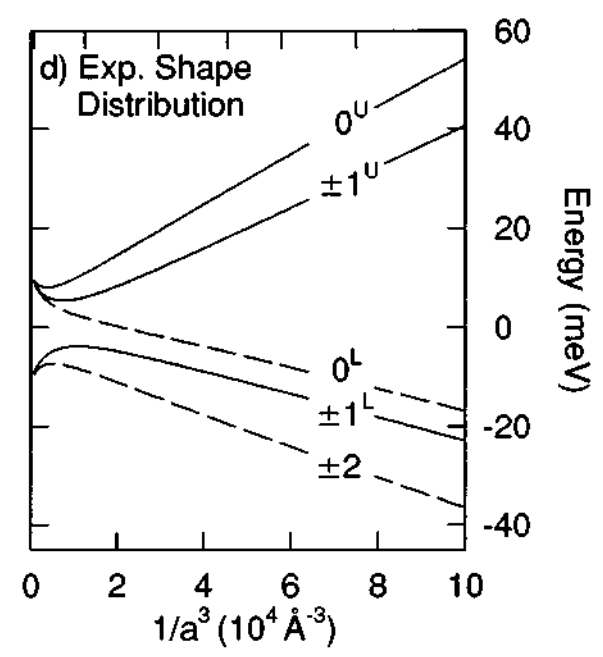
\includegraphics[width=0.5\textwidth]{./Chapter1/efs_efros.png}
\caption[Size-dependence of exciton fine structure in CdSe nanocrystals.]{Size-dependence of the exciton fine structure for the $1S_{3/2}-1S_e$ (band edge) exciton in CdSe NCs. Reproduced from the work by Efros \emph{et al.} \cite{PhysRevB.54.4843}, who utilized a multiband effective mass model with sizes and shape asymmetry derived from experimental measurements.}
\label{f:efs2}
\end{center}
\end{figure}

As shown in Figure \ref{f:efs2}, the splitting between exciton fine structure states in CdSe nanocrystals depends on NC size, a result which has been predicted theoretically and experimentally confirmed using low-temperature optical measurements \cite{PhysRevB.54.4843}. The implications of the exciton fine structure in CdSe are discussed further in Chapter 3.

\section{Carrier Cooling in Semiconductor Nanocrystals}

The intraband relaxation of excited charge carriers in semiconductor NCs has been a topic of significant interest owing to the theoretical prediction of dramatically slowed carrier cooling rates in comparison to bulk materials \cite{benisty1991intrinsic, bockelmann1990phonon}. In bulk semiconductors, intraband relaxation of hot carriers occurs on a roughly 1 ps timescale. This cooling occurs so rapidly due to the continuous energy bands exhibited by bulk, crystalline materials, which provide resonant electronic states for highly efficient electron-phonon scattering.  A general schematic of the carrier cooling process is displayed in Figure \ref{f:carrier_cooling1} \cite{nozik2001spectroscopy}. 

\begin{figure}
\begin{center}
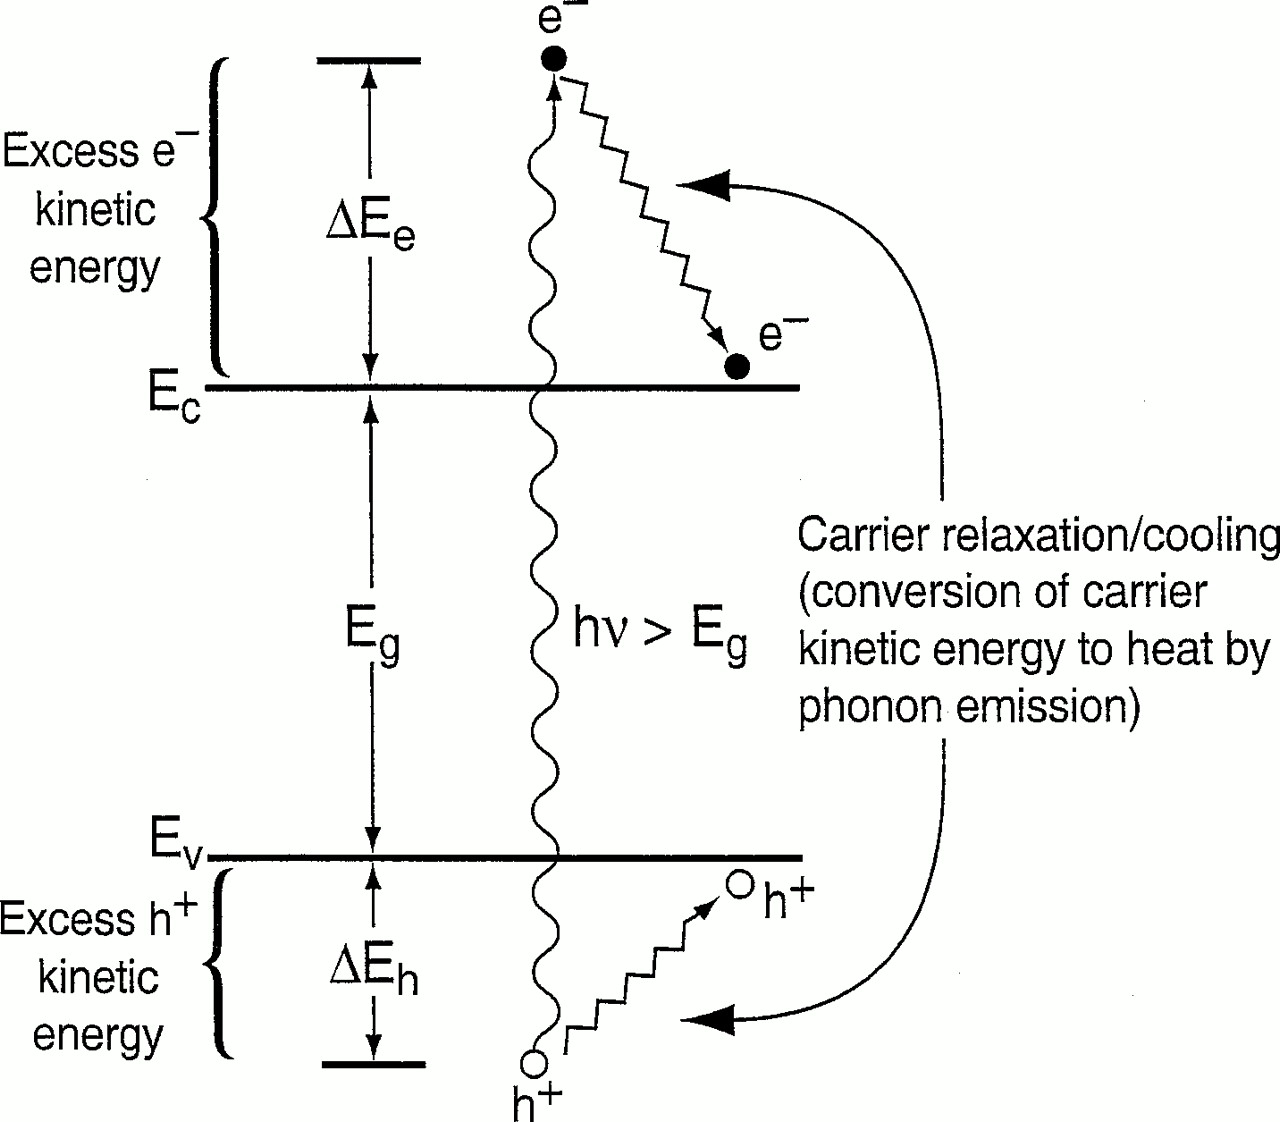
\includegraphics[width=0.5\textwidth]{./Chapter1/carrier_cooling.jpeg}
\caption[Schematic of phonon-assisted intraband carrier cooling in semiconductors.]{Subsequent to the creation of highly excited electrons and holes by absorption of an above gap photon, charge carriers relax to the conduction and valence band extrema ($E_c$ and $E_v$, respectively) by emitting phonons and heating the semiconductor lattice.}
\label{f:carrier_cooling1}
\end{center}
\end{figure}

In NCs, the discrete density of states arising from quantum confinement creates a scenario where the energetic spacing can exceed 10 times the LO phonon energy (typically on the order of $\sim$25 meV), which suggests that multi-phonon emission would be required to enable carrier relaxation. Such a multi-particle process would be much less efficient than cooling facilitated by single phonon emission, leading to the expectation of a "phonon bottleneck" with intraband carrier relaxation possibly taking up to a microsecond \cite{bockelmann1990phonon}. The prospect of a phonon bottleneck is enticing, as slowed carrier potentially offers benefits to many energy-related technologies. In particular, the ability to harvest hot carriers in photovoltaic cells would permit the utilization of above-gap solar photons to generate additional voltage. Alternatively, slowed carrier cooling would likely also benefit carrier multiplication processes, providing additional current. \par

Despite predictions of slowed carrier thermalization and the potential benefits of such a phenomenon, transient absorption measurements of carrier cooling relay subpicosecond-to-picosecond intraband relaxation times comparable to those exhibited by bulk materials \cite{PhysRevB.60.R2181, PhysRevLett.80.4028,PhysRevLett.96.057408}. Such rapid carrier transfer in NCs begins to suggest the involvement of other highly efficient relaxation processes, such as electron-to-hole energy transfer or energy transfer to surface-bound organic ligands exhibiting higher frequency vibrations \cite{pandey2008slow, guyot2005intraband}.\par

\begin{figure}
\begin{center}
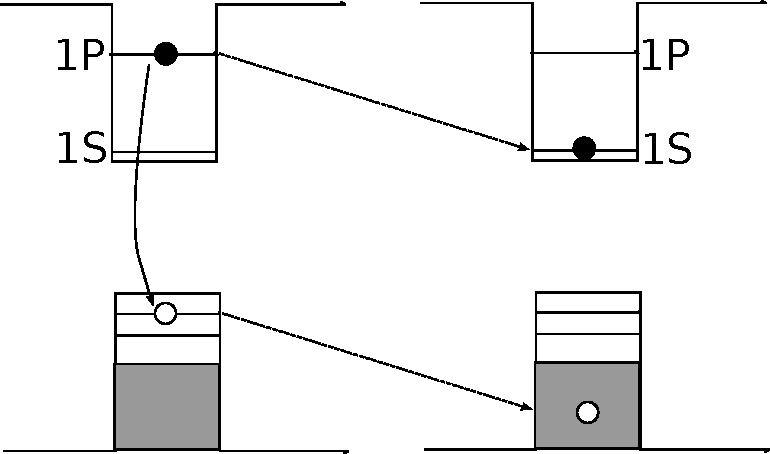
\includegraphics[width=0.5\textwidth]{./Chapter1/auger.pdf}
\caption[Schematic of Auger-like electron-to-hole energy transfer in NCs.]{Confinement enhanced, Auger-like energy transfer in NCs entails a highly excited electron (solid circle) resonantly transfering energy to the hole (open circle) \emph{via} the Coulomb interaction. This facilitates rapid electron cooling even in the presence of conduction band states with energetic separation well in excess of typical phonon energies. Holes, which are heavier, can still undergo phonon-assisted relaxation through the valence band.}
\label{f:carrier_cooling2}
\end{center}
\end{figure}

The dominant mechanism for rapid carrier cooling in NCs is theorized to be Auger-like energy transfer from the electron to the hole, which proceeds in the following fashion. Electrons, typically exhibiting a smaller effective mass than the hole, resonantly transfer energy uni-directionally \emph{via} a Coulombic interaction to holes. Subsequent to this energy transfer, the heavier holes, which experience a higher density of states, efficiently couple to phonons to relax to the band edge. Figure \ref{f:carrier_cooling2} graphically depicts the Auger-like energy transfer process, with the hole being excited into a "bulk"-like quasi-continuum of states at high energies, shown as a solid grey section of the valence band in the figure. While the theoretically predicted Auger-like energy transfer rates exhibit a size-dependence matching experimentally measured intraband relaxation times in NCs, the theory ultimately remains unproven, with more recent experimental results possibly challenging this interpretation. We explore this notion in detail in Chapter 2.

\section{Mechanisms of Heat Transport}
Another major focus of this thesis is the ultimate fate of phonons after they are generated by intraband carrier thermalization (and other means). As NCs become increasingly technologically relevant, it will become necessary to address the thermal management challenges inherent to this material class. While NCs exhibit remarkable, tunable optical and electronic properties, they present a greatly elevated surface-to-volume ratio which depresses the melting point relative to bulk materials \cite{goldstein1992melting}. Furthermore, even at temperatures below the NC melting point, processing such as sintering in NC films can alter the size-dependent optical properties and negatively affect performance \cite{drndic2002transport}. Finally, the chemical passivating layer on the surface renders NCs susceptible to damage mechanisms such as ligand decomposition and subsequent surface trap formation. \par

NCs and films comprised of them present unique challenges with regard to the study of thermal transport. Addressing some of these challenges is the focus of Chapter 3 of this thesis, and we elaborate on many NC-specific challenges there. Here, we review some of the basic theory of thermal transport in order to lay a foundation for the work presented in this thesis.

\subsection{Fourier's Law}
Heat conduction is an energy transfer process through a medium which is caused by a temperature difference due to the motion of heat carriers in that medium. Importantly, heat conduction requires a medium, and such processes are usually modeled on the basis of Fourier's Law \cite{chen2000particularities}:
\begin{equation}\label{eq:fourier1}
q = -\lambda\nabla T
\end{equation}
In Equation \ref{eq:fourier1}, $q$ is the heat flux, $\nabla T$ is the temperature gradient, and $\lambda$ is the thermal conductivity. Fourier's Law implicitly assumes diffusive heat transport mediated by the scattering of heat carriers in the material (phonons in semiconductors and insulators, while in metals electrons also exhibit significant heat capacity). Applying this theory to systems exhibiting structure or grain boundaries on the nanometer length scale is challenging, as typical phonon mean free paths exceed this length scale significantly \cite{chen2000particularities, cahill2003nanoscale}. As a result, one might intuitively expect shorter distances between scattering events as compared to bulk materials and commensurately reduced thermal conductivity. Indeed, this is generally the case \cite{cahill2003nanoscale}, and nanostructuring has emerged as a major paradigm in the rational design of thermoelectric materials exhibiting ultralow thermal conductivity \cite{doi:10.1021/cm902195j, Hsu06022004}. \par
Development of a complete model of nanoscale heat transport remains an extremely active area of research \cite{cahill2014nanoscale, france2014atomistic, merabia2014thermal, maznev2015boundary}. As we will see, even thermal transport at isolated, chemically-passivated interfaces presents significant outstanding experimental and theoretical challenges. As a starting point, it is reasonable to consider heat transport at an interface, as it is interfacial scattering which dominates heat transport in nanoscale systems. Extending Fourier's Law, we may write:
\begin{equation}\label{eq:fourier2}
q = G\Delta T
\end{equation}
In Eq. \ref{eq:fourier2}, $G$ is the interfacial thermal conductance and $\Delta T$ is the temperature change at the interface. Next, we present a microscopic theory of $G$ and comment on the difficulties associated with the analytical calculation of this term, highlighting the need for numerical simulations.

\subsection{Heat Transport at Interfaces}
As described above, systems presenting interfaces on length scales much less than typical phonon mean free paths will usually exhibit thermal transport dominated by interfacial thermal conductance. A theoretical model of interfacial thermal conductance begins with a microscopic expression for phonon flux at an interface. Figure \ref{f:ch1nano1} displays a diagram of the interface between two materials.

\begin{figure}
\begin{center}
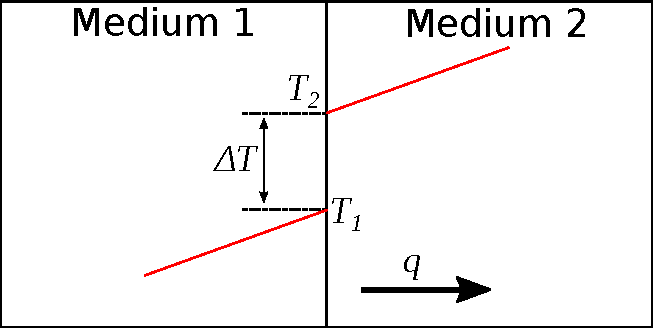
\includegraphics[width=0.5\textwidth]{./Chapter1/nanoscale1.pdf}
\caption[Diagram of thermal transport between interfaces.]{Model of interfacial thermal conductance \cite{PhysRevB.86.094303}. The red lines represent temperature profiles in each material, with a temperature jump shown at the interface. This discontinuity arises from different thermal conductivity in each material. The interfacial heat flux is given by $q$, and the direction of this flux by the arrow in medium 2.}
\label{f:ch1nano1}
\end{center}
\end{figure}

In the most general sense, we may naively write the following expression for phonon flux in the $z$ direction for an interface between two material regions designated $L$ and $R$ (Medium 1 and 2, respectively, in Fig. \ref{f:ch1nano1}) \cite{PhysRevB.80.165304}:
\begin{equation}\label{eq:nanoheat1}
\begin{split}
q =& \frac{1}{\left(2\pi\right)^3}\left[\int_L\sum_v^+ \hbar\omega(\vec{k},v)v_z(\vec{k}, v)\alpha_{L \rightarrow R}(\vec{k},v)f_L(\vec{k},v)\mathrm{d}\vec{k}\right. \\
&+ \left.\int_R\sum_v^- \hbar\omega(\vec{k},v)v_z(\vec{k}, v)\alpha_{R \rightarrow L}(\vec{k},v)f_R(\vec{k},v)\mathrm{d}\vec{k}\right]
\end{split}
\end{equation}

Equation \ref{eq:nanoheat1} simply sums up, for each phonon polarization (or vibrational mode $v$ in a molecular eigenstate picture) $v$, the energy of a phonon having frequency $\omega$ multiplied by its velocity in the $z$ direction, $v_z$, an energy-dependent transmission coefficient $\alpha$ (with energy-dependence entering via the dependence on phonon wavevector $\vec{k}$), and a phonon distribution function $f$, which accounts for thermal population of the various modes. Each sum is integrated over the first Brillouin zone of that particular lead ($L$ or $R$). The factor $1/\left(2\pi\right)^3$ accounts for the reciprocal space volume in the medium.  Given exact forms of the transmission coefficient and the phonon distribution function, this expression for phonon flux is exact, however, exact expressions for these terms are difficult to obtain for heterogeneous interfaces. Varying levels of approximiations exist, the most relevant of which we will describe here, along with specific issues related to nanoscale thermal transport.\par

The most straightforward approximation is to model the phonon distribution function, $f$, with the equilibrium Bose-Einstein distribution, i.e.:
\begin{equation}\label{eq:nanoheat2}
f_{L/R} = f_{eq}(\omega, T) = \frac{1}{e^{-\hbar\omega/k_BT} - 1}
\end{equation}
In Eq. \ref{eq:nanoheat2}, $k_B$ is Boltzmann's constant and $T$ is temperature. The use of an equilibrium distribution function to describe an inherently non-equilibrium process (heat transport) leads to the significant contradiction that the interface between two identical materials is predicted to have a finite interfacial thermal conductance. To demonstrate this, we note that flux must vanish at equilibrium, i.e. $q = 0$. Then, the two terms on the right-hand side of Eq. \ref{eq:nanoheat1} must vanish:
\begin{equation}\label{eq:nanoheat3}
\begin{split}
\int_L\sum_v^+ \hbar\omega(\vec{k},v)v_z(\vec{k}, v)\alpha_{L \rightarrow R}(\vec{k},v)f_{eq}(\omega, T_L)\mathrm{d}\vec{k} \\
= -\int_R\sum_v^- \hbar\omega(\vec{k},v)v_z(\vec{k}, v)\alpha_{R \rightarrow L}(\vec{k},v)f_{eq}(\omega, T_R)\mathrm{d}\vec{k}
\end{split}
\end{equation}
We can then simplify Eq. \ref{eq:nanoheat1} to involve integration over only one side of the interface:
\begin{equation}\label{eq:nanoheat4}
q = \frac{1}{\left(2\pi\right)^3}\int_L\sum_v^+ \hbar\omega(\vec{k},v)v_z(\vec{k}, v)\alpha_{L \rightarrow R}(\vec{k},v)\left[f_{eq}(\omega, T_L) - f_{eq}(\omega, T_R)\right]\mathrm{d}\vec{k}
\end{equation}
Using Fourier's Law (described in the previous section), this can be converted to an interfacial thermal conductance.
\begin{equation}\label{eq:nanoheat5}
G = \frac{q}{T_L - T_R} = \frac{1}{\left(2\pi\right)^3}\int_L\sum_v^+ \hbar\omega(\vec{k},v)v_z(\vec{k}, v)\alpha_{L \rightarrow R}(\vec{k},v)\left[\frac{f_{eq}(\omega, T_L) - f_{eq}(\omega, T_R)}{T_L - T_R}\right]\mathrm{d}\vec{k}
\end{equation}
In the equilibrium limit, $T_L \rightarrow T_R$, and we arrive at the Landauer interfacial thermal conductance \cite{landauer1970electrical}:
\begin{equation}\label{eq:nanoheat6}
G_{eq} = \frac{1}{\left(2\pi\right)^3}\int_L\sum_v^+ \hbar\omega(\vec{k},v)v_z(\vec{k}, v)\alpha_{L \rightarrow R}(\vec{k},v)\left[\frac{\partial f_{eq}\left(\omega, T_R\right)}{\partial T}\right]\mathrm{d}\vec{k}
\end{equation}
As noted above, Eq. \ref{eq:nanoheat6} predicts a \emph{finite} thermal conductance between identical materials ($\alpha_{L \rightarrow R} = 1$), which is clearly unphysical. To address this issue, we may utilize the Boltzmann transport equation under relaxation time approximation (RTA), which gives an expression for the non-equilibrium phonon distribution function \cite{ziman1960electrons}.  In the RTA, the time dependence of the phonon distribution function, $f$, is given by Equation \ref{eq:nanoheat7}:
\begin{equation}\label{eq:nanoheat7}
\frac{\partial f_i}{\partial t} + v_i \cdot \nabla f_i = \frac{f_i - f_{eq}}{\tau_i\left(\omega\right)}
\end{equation}
In Eq. \ref{eq:nanoheat7}, $\tau_i$ is the mode-dependent relaxation time, which is a measure of the time taken for a non-equilibrium phonon population to return to its equilibrium state. A solution of this differential equation is given by Equation \ref{eq:nanoheat8}:
\begin{equation}\label{eq:nanoheat8}
f_i\left(\vec{r}\right) = f_{eq}\left[T(\vec{r})\right] - \tau_i\left(\frac{\partial f_{eq}}{\partial T}\right)v_i \cdot \nabla T
\end{equation}
Inserting the new distribution function (Eq. \ref{eq:nanoheat8}) into the expression for flux (Eq. \ref{eq:nanoheat1}) and grouping the terms into equilibrium and non-equilibrium branches, we have:
\begin{equation}\label{eq:nanoheat9}
\begin{split}
q &= G_{eq} \cdot (T_L - T_R) - \int_L\sum_{v}^{+}\hbar\omega(\vec{k},v)v_z(\vec{k},v)^2\alpha_{L\rightarrow R}(\vec{k},v)\tau_L\left(\frac{\partial f_{eq}}{\partial T}\right)\left(\frac{\partial f_{eq}}{\partial z}\right)_L \\
&- \int_R\sum_{v}^{+}\hbar\omega(\vec{k},v)v_z(\vec{k},v)^2\alpha_{R\rightarrow L}(\vec{k},v)\tau_R\left(\frac{\partial f_{eq}}{\partial T}\right)\left(\frac{\partial f_{eq}}{\partial z}\right)_R
\end{split}
\end{equation}
Equation \ref{eq:nanoheat9} accounts for the inherently non-equilibrium nature of phonon flux, but the transmission coefficients $\alpha$ and phonon lifetimes $\tau_i$ remain unknown in general. Transmission coefficients are typically calculated using one of two approximate models: the acoustic mismatch model (AMM) and the diffuse mismatch model (DMM). The key difference between these two models is the central assumption made regarding the nature of phonon scattering, as conceptualized in Figure \ref{f:ch1nano2}. 

\begin{figure}
\begin{center}
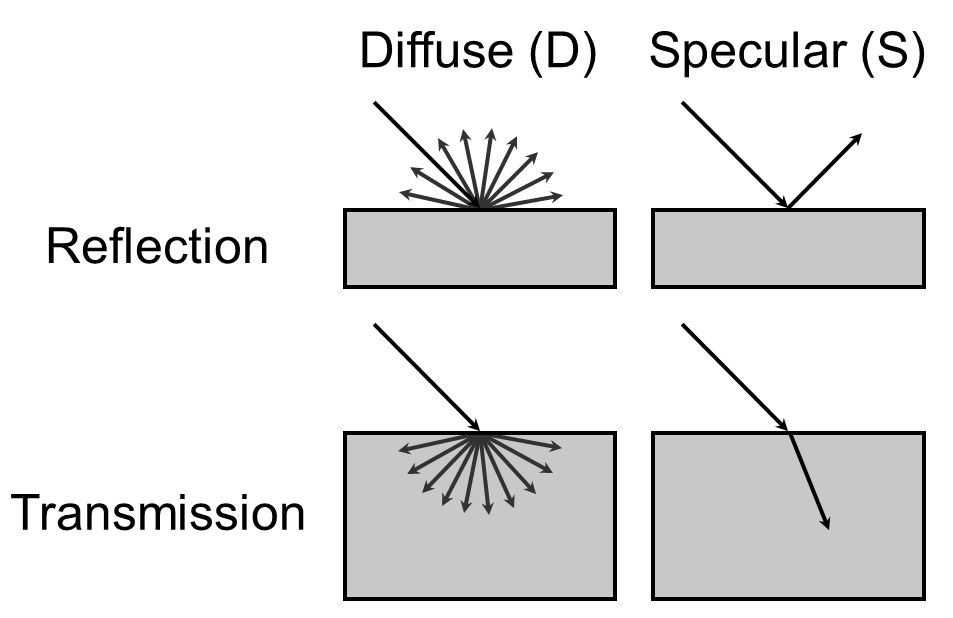
\includegraphics[width=0.5\textwidth]{./Chapter1/nanoscale2.png}
\caption[Comparison of specular and diffusive scattering processes.]{Comparison of specular and diffusive reflection and transmission. In general, specular scattering occurs from interfaces which are "smooth" with respect to the incoming wave, and the reflected/transmitted waves will retain memory of their momenta prior to scattering. Diffuse scattering occurs from "rough" interfaces, causing completely random scattering with no dependence on the history of the incoming wave.}
\label{f:ch1nano2}
\end{center}
\end{figure}

\subsubsection{The Acoustic Mismatch Model} In the AMM, phonons propagating towards an interface are assumed to interact with that interface as a sharp discontinuity of acoustic impedance, $Z_i$, where:
\begin{equation}\label{eq:nanoheat10}
Z_i = \rho_ic_i
\end{equation}
In the above equation, $\rho_i$ is the mass density of medium $i$ and $c_i$ is the acoustic velocity. Phonons may be reflected by the interface or refracted on the other side of it by following an equivalent of Snell's Law, given by Equation \ref{eq:nanoheat11}:
\begin{equation}\label{eq:nanoheat11}
\frac{\sin{\theta_1}}{c_1} = \frac{\sin{\theta_2}}{c_2}
\end{equation}
In Eq. \ref{eq:nanoheat11}, $\theta_1$ and $\theta_2$ are the incident and refraction angles, respectively. Several assumptions are implicit in utilizing Snell's Law here. Firstly, it is also assumed that phonon polarization is conserved. Secondly, the AMM as presented here assumes that interfacial scattering is elastic; that is, phonons conserve their frequency. As a consequence, phonons having a frequency above the Debye frequency of the softer (that is, having a lower Debye frequency) material are confined in the harder (that is, having a higher Debye frequency) material and do not cross the interface ($\alpha \rightarrow 0$). For phonons with frequencies smaller than the Debye frequency of the softer material, the transmission coefficient is derived from Snell's Law:
\begin{equation}\label{eq:nanoheat12}
\alpha_{1 \rightarrow 2}  = \frac{4Z_1Z_2\mu_1\mu_2}{\left(Z_1\mu_1 + Z_2\mu_2\right)^2} 
\end{equation}
In Eq. \ref{eq:nanoheat12}, $\mu_i = \cos{\theta_i}$. The derivation of Eq. \ref{eq:nanoheat12} from Snell's Law is straightforward, albeit lengthy, and was originally published by Little \cite{little1959transport}, to whose work the reader is referred for the full derivation.  
\subsubsection{The Diffuse Mismatch Model}
When phonon wavelengths are comparable to or smaller than interfacial roughness, phonons scattering at the interface are assumed to lose all information about the medium from which they originated. Thus, the probability of phonon transmission from medium 1 to 2 is equal to the probability that a phonon experiences a reflection in medium 2, i.e.
\begin{equation}\label{eq:nanoheat13}
\alpha_{1 \rightarrow 2} = 1 - \alpha_{2 \rightarrow 1}
\end{equation}
Following the derivation of Swartz and Pohl \cite{RevModPhys.61.605} we arrive at the DMM expression for the transmission coefficient:
\begin{equation}\label{eq:nanoheat13}
\alpha_{1 \rightarrow 2} = \frac{c_2g_2\left(\omega\right)}{c_1g_1\left(\omega\right) + c_2g_2\left(\omega\right)}
\end{equation}
In Eq. \ref{eq:nanoheat13}, $g_i\left(\omega\right)$ is the phonon density of states in medium $i$. Note that the DMM also assumes that high-frequency phonons are in confined the harder material \cite{PhysRevB.86.094303}. 
\subsubsection{Approximations for Phonon Lifetime}
The simplest approximation for the phonon lifetime, originally proposed by Callaway \cite{PhysRev.113.1046}, is the assumption that Umklapp scattering processes dominate the phonon relaxation. Umklapp scattering is a type of phonon-phonon scattering wherein scattered phonons exhibit a wavevector exceeding the boundary of the first Brillouin zone. This necessarily alters the direction of flux for scattered phonons and is partly responsible for the diffusive nature of phonon transport in bulk materials. Within the Callaway model, phonon lifetimes have the following dependence:
\begin{equation}\label{eq:nanoheat13}
\tau_i(\omega) = A_i\omega^{-2}
\end{equation}
In Equation \ref{eq:nanoheat13}, $A_i$ is collection of material-specific, temperature dependent parameters \cite{PhysRevB.86.094303}, and $\omega$ is the phonon frequency. While this approximation can work well for bulk materials and isolated crystalline interfaces, attempts to apply this model to nanostructured systems yield significant deviation of experimental results from the theory at elevated temperatures \cite{liu2006thermal}. Considering the dominance of interfacial phenomena at the nanometer length scale, the Callaway model is unlikely to suitably model phonon lifetimes for the systems studied in this thesis. 
\subsubsection{Application to Chemically-passivated, Nanometer-scale Systems}
The assumptions inherent in the models described above make them difficult to apply directly to the systems of interest here, which typically present chemically-passivated (usually by long-chain organic molecules such as alkylamines, alkanethiols, and organophosphorous species) interfaces on nanometer length scales. In particular, both the AMM and DMM require knowledge of the material sound velocity, which is typically poorly characterized for organic monolayers. Furthermore, at ambient temperatures, Umklapp scattering processes do not necessarily determine phonon relaxation times. While more advanced models of phonon lifetime exist based on anharmonic lattice dynamics \cite{PhysRevB.80.165304}, the effects of nanoscale confinement and atomic-scale disorder (introduced by the chemical passivating layer) on these models is generally unknown. Thus, we focus our theoretical efforts on molecular dynamics simulations, which make no assumptions regarding the nature of phonon scattering and can account for chemical details in a fully atomistic way. We elaborate on some of these considerations in Chapter 3.
\section{Outline}
The work in this thesis is divided into two major categories: Thermal processes in semiconductor nanocrystals and photoluminescence (PL) in group-IV semiconductor nanocrystals. In Chapter 2, we review the experimental details of ultrafast optical spectroscopy, necessary to characterize the carrier dynamics exhibited by these materials in real time. Next, we explore the earliest stages of heat generation - energy dissipation by photoexcited charge carriers. We apply a recently developed technique, femtosecond stimulated Raman spectroscopy, to directly observe, for the first time, phonon generation as a result of carrier cooling in CdSe nanocrystals. We find a lack of size-dependence in phonon generation dynamics, consistent with size-independent hole-phonon coupling in these materials. In addition to laying the groundwork for more advanced studies of vibrational energy flow in NC systems, these results lend credence to as-yet unproven theories regarding confinement enhanced, Auger-like electron-to-hole energy transfer in II-VI semiconductor nanocrystal compositions. \par
In Chapter 3, we focus on the fate of phonons after they are generated. First, we characterize a previously-unexplained ultrafast decay feature evident in the low-temperature PL dynamics of matrix-embedded CdSe nanocrystals. Utilizing streak camera measurements and a size-series of CdSe NCs, we are able to attribute this decay feature to rapid emission facilitated by non-equilibrium acoustic phonons generated by carrier cooling. We further associate the decay of this PL feature with acoustic phonon outflow and demonstrate that this optical signature can be used to characterize thermal transport rates at the NC-matrix interface. Next, we examine the interfacial thermal transport process for chemically-passivated NCs with atomistic resolution using molecular dynamics (MD) simulations. Specifically, we utilize a recently-developed MD method well-suited to the study of transport at heterogeneous, acoustically mismatched interfaces. We demonstrate that thermal transport at the semiconductor/solvent interface is significantly enhanced by the presence of surface ligands and that the underlying structure of the exposed semiconductor surface places fundamental limits on thermal conductance because it controls maximal ligand grafting density. \par
In Chapter 4, several chemical methods for manipulating thermal processes in NCs are explored. Primarily, we utilize the optical signature of thermal transport detailed in Chapter 3 to characterize a range of NCs presenting a fixed core size with increasingly thick, optoelectronically inert shells. We demonstrate that inert shell growth permits separate tuning of the thermal and optical properties of NCs. We also briefly report on theoretical work done in support of larger experimental efforts. Specifically, we discuss the possibility that two new surface termination motifs (passivation by small, inorganic capping ligands and covalently-bound ligands) may confer thermal stability benefits similar to those provided by shell growth, but without confining one or both charge carriers to the NC core (which hinders their application in technologies requiring carrier mobility). \par
Chapter 5 contains the second major category in this thesis. We report a detailed experimental and theoretical investigation of PL enhancement in silicon nanocrystals. Radiative recombination becomes efficient in nanometer-scale silicon materials, but the mechanism of enhanced photon emission has long been contested, with a variety of mechanisms each having a substantial body of supporting literature. In particular, efficient PL from silicon NCs has been attributed to relaxation of momentum-conservation requirements by translational symmetry loss, emission from surface oxide species, direct-gap emission from hot carriers, and quasidirect emission from band-edge states broadened in $k$-space by ligand species. We utilize pressure-dependent optical spectroscopy and find that the pressure-induced shift of steady-state PL from silicon NCs matches the band-edge pressure coefficient of bulk Si. Combined quantum/classical simulations of silicon NCs under pressure yield a similar dependence of the NC energy gap and further confirm that the band-edge states are delocalized throughout the NC rather than confined to a surface state. Taken together, these results strongly suggest that band-edge PL in silicon NCs remains indirect in character despite substantial quantum confinement. Next, we explore high-energy, short-lived PL using time-resolved PL spectroscopy and Raman spectroscopy. We investigate PL dynamics as a function of NC size and lattice crystallinity and, in conjunction with molecular dynamics simulations and TEM characterization, attribute high-energy PL to an emissive amorphous surface layer. \par
Finally, in Chapter 6, we present structural characterization of group-IV nanocrystals at elevated pressures. While the main focus of our pressure-dependent work was on elucidating the origin of light emission in these materials, the pressure-dependent structural properties of NCs are interesting enough to merit some separate discussion. We present pressure-dependent XRD of both silicon and Ge nanocrystals. Interestingly, we find these particles to exhibit compressibility matching the bulk phase, in contrast to most other NC compositions. We also analyze molecular dynamics simulations of the pressurization process to provide insight regarding the nature of pressure-induced structural changes in these materials.